% Important: If latex complains about unicode characters,
% please use "\usepackage[utf8x]{inputenc}" in your preamble
% You can change the size of the picture by putting it into the construct:
% 1) \resizebox{10cm}{!}{"below picture"} to scale horizontally to 10 cm
% 2) \resizebox{!}{15cm}{"below picture"} to scale vertically to 15 cm
% 3) \resizebox{10cm}{15cm}{"below picture"} a combination of above two
% It is not recomended to use the scale option of the tikzpicture environment.
 \resizebox{7cm}{!}{
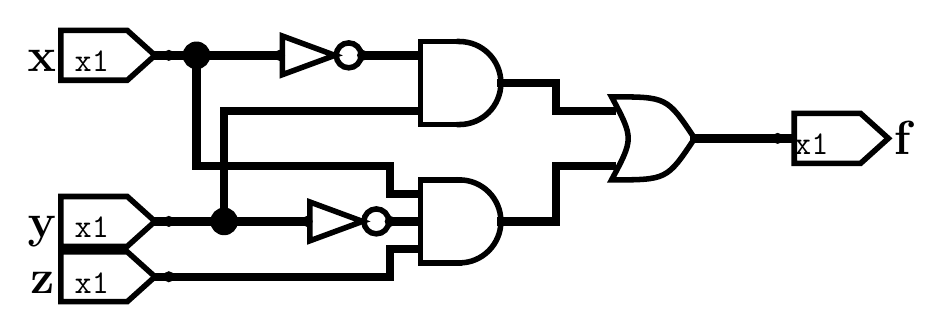
\begin{tikzpicture}[x=1pt,y=-1pt,line cap=rect]
\def\logisimfontA#1{\fontfamily{cmr}{#1}} % Replaced by logisim, original font was "SansSerif"
\def\logisimfontB#1{\fontfamily{cmtt}{#1}} % Replaced by logisim, original font was "Monospaced"
\definecolor{custcol_0_0_0}{RGB}{0, 0, 0}
\definecolor{custcol_ff_ff_ff}{RGB}{255, 255, 255}
\draw [line width=3.0pt, custcol_0_0_0 ]  (246.0,45.0) -- (276.0,45.0) ;
\draw [line width=3.0pt, custcol_0_0_0 ]  (126.0,15.0) -- (146.0,15.0) ;
\draw [line width=3.0pt, custcol_0_0_0 ]  (136.0,75.0) -- (146.0,75.0) ;
\draw [line width=3.0pt, custcol_0_0_0 ]  (96.0,15.0) -- (66.0,15.0) -- (66.0,55.0) -- (136.0,55.0) -- (136.0,65.0) -- (146.0,65.0) ;
\draw [line width=3.0pt, custcol_0_0_0 ]  (106.0,75.0) -- (76.0,75.0) -- (76.0,35.0) -- (146.0,35.0) ;
\fill [line width=3.0pt, custcol_0_0_0]  (76.0,75.0) ellipse (5.0 and 5.0 );
\fill [line width=3.0pt, custcol_0_0_0]  (66.0,15.0) ellipse (5.0 and 5.0 );
\draw [line width=2.0pt, custcol_0_0_0] (161.0,40.0) arc (90.0:-90.0:15.0 and 15.0 );
\draw [line width=2.0pt, custcol_0_0_0 ]  (161.0,10.0) -- (147.0,10.0) -- (147.0,40.0) -- (161.0,40.0) ;
\draw [line width=3.0pt, custcol_0_0_0 ]  (176.0,25.0) -- (196.0,25.0) -- (196.0,35.0) -- (216.0,35.0) -- (216.0,35.0) ;
\draw [line width=3.0pt, custcol_0_0_0 ]  (176.0,75.0) -- (196.0,75.0) -- (196.0,55.0) -- (216.0,55.0) -- (216.0,55.0) ;
\draw [line width=2.0pt, custcol_0_0_0 ]  (246.0,45.0) .. controls  (236.0,30.0)  ..  (216.0,30.0) .. controls  (224.0,45.0)  ..  (216.0,60.0) .. controls  (236.0,60.0)  ..  (246.0,45.0) -- cycle ;
\draw [line width=3.0pt, custcol_0_0_0 ]  (280.0,45.0) -- (277.0,45.0) ;
\draw [line width=2.0pt, custcol_0_0_0 ]  (306.0,36.0) -- (316.0,45.0) -- (306.0,54.0) -- (282.0,54.0) -- (282.0,36.0) -- cycle;
\logisimfontB{\fontsize{12pt}{12pt}\selectfont\node[inner sep=0, outer sep=0, custcol_0_0_0, anchor=base west] at  (282.0,51.0)  {x1};}
\logisimfontA{\fontsize{16pt}{16pt}\fontseries{bx}\selectfont\node[inner sep=0, outer sep=0, custcol_0_0_0, anchor=base west] at  (318.0,51.0)  {f};}
\fill [line width=2.0pt, custcol_0_0_0]  (276.0,45.0) ellipse (2.0 and 2.0 );
\draw [line width=2.0pt, custcol_0_0_0 ]  (116.0,15.0) -- (97.0,8.0) -- (97.0,22.0) -- cycle;
\draw [line width=2.0pt, custcol_0_0_0]  (121.0,15.0) ellipse (4.5 and 4.5 );
\fill [line width=2.0pt, custcol_0_0_0]  (126.0,15.0) ellipse (2.0 and 2.0 );
\fill [line width=2.0pt, custcol_0_0_0]  (96.0,15.0) ellipse (2.0 and 2.0 );
\draw [line width=2.0pt, custcol_0_0_0 ]  (126.0,75.0) -- (107.0,68.0) -- (107.0,82.0) -- cycle;
\draw [line width=2.0pt, custcol_0_0_0]  (131.0,75.0) ellipse (4.5 and 4.5 );
\fill [line width=2.0pt, custcol_0_0_0]  (136.0,75.0) ellipse (2.0 and 2.0 );
\fill [line width=2.0pt, custcol_0_0_0]  (106.0,75.0) ellipse (2.0 and 2.0 );
\draw [line width=2.0pt, custcol_0_0_0] (161.0,90.0) arc (90.0:-90.0:15.0 and 15.0 );
\draw [line width=2.0pt, custcol_0_0_0 ]  (161.0,60.0) -- (147.0,60.0) -- (147.0,90.0) -- (161.0,90.0) ;
\draw [line width=3.0pt, custcol_0_0_0 ]  (51.0,15.0) -- (56.0,15.0) -- (66.0,15.0) ;
\draw [line width=2.0pt, custcol_0_0_0 ]  (41.0,24.0) -- (51.0,15.0) -- (41.0,6.0) -- (17.0,6.0) -- (17.0,24.0) -- cycle;
\logisimfontB{\fontsize{12pt}{12pt}\selectfont\node[inner sep=0, outer sep=0, custcol_0_0_0, anchor=base west] at  (22.0,21.0)  {x1};}
\logisimfontA{\fontsize{16pt}{16pt}\fontseries{bx}\selectfont\node[inner sep=0, outer sep=0, custcol_0_0_0, anchor=base west] at  (5.0,21.0)  {x};}
\fill [line width=2.0pt, custcol_0_0_0]  (56.0,15.0) ellipse (2.0 and 2.0 );
\draw [line width=3.0pt, custcol_0_0_0 ]  (51.0,75.0) -- (56.0,75.0) -- (76.0,75.0) ;
\draw [line width=2.0pt, custcol_0_0_0 ]  (41.0,84.0) -- (51.0,75.0) -- (41.0,66.0) -- (17.0,66.0) -- (17.0,84.0) -- cycle;
\logisimfontB{\fontsize{12pt}{12pt}\selectfont\node[inner sep=0, outer sep=0, custcol_0_0_0, anchor=base west] at  (22.0,81.0)  {x1};}
\logisimfontA{\fontsize{16pt}{16pt}\fontseries{bx}\selectfont\node[inner sep=0, outer sep=0, custcol_0_0_0, anchor=base west] at  (5.0,81.0)  {y};}
\fill [line width=2.0pt, custcol_0_0_0]  (56.0,75.0) ellipse (2.0 and 2.0 );
\draw [line width=3.0pt, custcol_0_0_0 ]  (51.0,95.0) -- (56.0,95.0) -- (136.0,95.0) -- (136.0,85.0) -- (146.0,85.0) ;
\draw [line width=2.0pt, custcol_0_0_0 ]  (41.0,104.0) -- (51.0,95.0) -- (41.0,86.0) -- (17.0,86.0) -- (17.0,104.0) -- cycle;
\logisimfontB{\fontsize{12pt}{12pt}\selectfont\node[inner sep=0, outer sep=0, custcol_0_0_0, anchor=base west] at  (22.0,101.0)  {x1};}
\logisimfontA{\fontsize{16pt}{16pt}\fontseries{bx}\selectfont\node[inner sep=0, outer sep=0, custcol_0_0_0, anchor=base west] at  (6.0,101.0)  {z};}
\fill [line width=2.0pt, custcol_0_0_0]  (56.0,95.0) ellipse (2.0 and 2.0 );
\end{tikzpicture}
}